% %%% Time-stamp: <2024-01-03 13:22:46 vladimir>
% %%% Copyright (C) 2019-2024 Vladimir G. Ivanović
% %%% Author: Vladimir G. Ivanović <vladimir@acm.org>
% %%% ORCID: https://orcid.org/0000-0002-7802-7970

\chapter{Discussion}%
\label{ch:discussion}%
\noindent\bigskip%

This chapter addresses this dissertation's research question:
\medskip%
\begin{quote}\OnehalfSpacing
  Has Rocketship structured itself to earn a return for its founders and investors, focusing especially on its real estate transactions?
\end{quote}\index{research question}
The chapter looks more closely at the research question and summarizes the key findings of this research. It then discusses what kind of evidence would confirm or disconfirm the research question. It looks at three well-known approaches to making arguments for or against a proposal or policy and uses those approaches to make the case that Rocketship has in fact organized itself to make money and that real estate is the vehicle it uses. The two final sections discuss what policy issues are raised during the examination of the data and the evidence, what further research is warranted. Lastly, this dissertation makes a brief conclusion.

\section{The Research Question}%
\label{sec:research-question}\indent%

This dissertation's research question, is really asking three questions:
\begin{enumerate}
  \item Has Rocketship structured itself to make money?
  \item If so, is real estate Rocketship's chosen vehicle?
  \item Is this Rocketship's intent?
\end{enumerate}

\section{Key Findings}%
\label{sec:summary-key-findings}\indent%

This dissertation's epigraph is \textit{Cui bono?} who benefits? In particular, who benefits from Rocketship's structure and activities?

After a careful examination of Rocketship's finances, a key finding is that no evidence of illegal activity was uncovered in Rocketship's \textit{publicly available} financial documents. This is fortunate, because California is notorious for charter school fraud. Nine years ago, \textcite{CPD2015} found \$81M in fraud, and in 2019, a single online charter school was discovered to have defrauded the State of California of \$400M. The report, \citetitle{CPD2015} estimated in 2015 that ``\ldots{} [t]he vast majority of this fraud perpetuated by charter officials will go undetected because California lacks the oversight necessary to identify the fraud.'' \parencite[2]{CPD2015}. With tens billions of dollars of funding for charter schools in California alone coupled with lax oversight, the temptation for fraud must be great. 

Rocketship does have some questionable expenditures, namely \$7.5M spent on travel in 2019–2022. This is a large sum, and should be investigated.

If no illegal activities were detected,  who actually benefits from Rocketship's growth in net assets?

\section{Arguments Which Answer the Research Question}%
\label{sec:appr-answ-rese-quest}\indent%

The next two sections each present a different style answer to this dissertation's research question. The first follows rules defined by Anatol Rapoport, a [mathematical] game theorist, who sought to increase understanding and avoid defensive responses. \citefirstlastauthor{Dennett2013} reformulated them in his book \citetitle{Dennett2013} \parencite{Dennett2013}. These are referred to in the literature as Rappaport's Rules. The second style was created by Stephen Toulmin, a British philosopher interested in moral reasoning. He developed a method for making practical arguments where ethics and morality played a role. Arguments made in this style are called Toulmin arguments.

Note that neither Rappaport nor Toulmin claim that their argument styles are logically rigorous; they are just a way articulating a point of view in a cohesive manner which fosters understanding and an exchange of ideas rather than descending into shouting, \textit{ad hominem} attacks, or a shutdown of communication.

\subsection{Rappaport's Rules}%
\label{sec:rappaports-rules}\indent%

Rappaport's rules for arguing are:
\begin{enumerate}[topsep=0.3\baselineskip,itemsep=0.25\baselineskip]
  \item Re-express your target’s position so clearly, vividly, and fairly that your target says, “Thanks, I wish I’d thought of putting it that way.”
  \item List any points of agreement (especially if they are not matters of general or widespread agreement).
  \item Mention anything you have learned from your target.
  \item Only then present your criticism.
\end{enumerate}
\medskip

Rocketship, following the Rappaport model, could potentially argue:
\begin{enumerate}[topsep=0.3\baselineskip,itemsep=0.25\baselineskip]
  \item Public schools, in areas of poverty, for whatever reason(s), fail to educate their students well, and they educate students of color especially poorly. We (Rocketship) aim to change this by a combination of focus, targeted intervention, and technology. We are focused on doing whatever it takes to raise the educational attainment of our students, and we focus day in and day out on this one goal. Our pedagogy has two major aspects: We monitor and target with specialize intervention students who are not doing as well as we would like, and we use technology (computer-aided instruction) to tailor instruction to a specific child's needs at exactly the time they need intervention.\\
  We believe that, by controlling our facilities, we can remove a serious distraction that comes with sharing facilities with a public school district. Not only are we not beholden to the whims of the public school district, but we do no have to spend time preparing year after year a Proposition 39 facilities request. We are never embroiled in petty disputes about interactions between public school students and our students because they simply never arise. Our results speak for themselves. All of our schools do better than their surrounding district and do better than the California average.
\end{enumerate}

A response to Rocketship's argument, again following Rappaport's model might be:
\begin{enumerate}[topsep=0.3\baselineskip,itemsep=0.25\baselineskip,resume]
  \item Although it is true that some public school districts have failed in their primary duty to educate children, this could be attributed to chronic underfunding and to local and state governments tolerating, and often abetting conditions that do not exist in suburbia. Staying the course, however, is not an option because doing the same thing over and over and expecting different results is not likely to be successful, now or ever.
  Further, providing separate facilities for children as Rocketship does rather than forced sharing is more likely to be successful than otherwise. Being able to control the school environment brings stability the classroom.

  \item Starting and operating a charter school is not for the faint of heart. Funding for both operation and for facilities is hard to come by, and must be procured before a single student arrives on campus. Facilities need to be constructed or modified well before classes begin. Children need to be enrolled, and parents need to be persuaded to help out. Juggling priorities, contingencies, and expectations is a full-time task, and it shows when the topics of board committee (executive, business, achievement, development) meetings are looked at.

  \item However, even given items 1–3 above, there are some areas where criticism, some of it quite severe, is warranted.

\begin{itemize}[topsep=0.125\baselineskip,itemsep=0.25\baselineskip]
    \item Even taking into consideration the acknowledged need for independent facilities, Rocketship spends an inordinate amount of time on topics that are not academic in focus. One can see this in the topic areas of its board committees, where only one of four has to do with academic achievement.
      \item Rocketship short-changes current students in order to create future students by allocating 20\% of revenue to facilities. Although this is legal, I suspect that the California Legislature did not expect one charter school to be begetting another, just as the Legislature didn't anticipate the damage that for-profit charter school chains or virtual charter schools would do.
      The percentage of revenue that Rocketship spends on administration (i.e. management), is unusually high at 14\% in 2022 \parencite[38]{RSEA2022}. General administrative expenses in public school districts are in the 5\% to 10\% range. So, immediately 35\% of revenue is siphoned off and does not go directly to educating children.
      \item Teachers at Rocketship schools in Santa Clara county have much less experience and are paid substantially less than, say, teachers in the San José Unified School District. If we believe that teachers are a key factor in delivering a quality education, then what kind of teachers Rocketship hires and how much it pays them are important determinants of the quality of the teaching staff and hence how well Rocketship educates its children. The evidence is not encouraging.
      \item Rocketship has exaggerated how well its students do compared to public school students. The size of the discrepancy is 4× to 5× larger than what is reported in the literature. A possible explanation for this difference is that Rocketship is trying to convince people that they are both committed to ``eliminating the achievement gap in our lifetime'' and more importantly, successful at it.\\
      According to the latest \citetitle{SCCOE2014}, comparing the percentage of Rocketship students who ``met/exceeded standards'' on the Smarter Balanced Summative Assessments (SBAC) test in English Language Arts (ELA) during the 2021-22 school year, only a single Rocketship school (out of eight Santa Clara County authorized schools) did better than public school students in Santa Clara County. In mathematics, the number of schools who did better was actually less than one; it was zero.\\
      Moving on to comparing how Rocketship schools did against state public schools, only one school exceeded the state average in ELA—by a single percentage point. Rocketship did better in mathematics: Five schools exceeded the state average in Mathematics. Granted, these results are not as bad as ACE Empower that managed only 19\% met or exceeded standards in ELA and 11\% in Mathematics, but for a chain of schools whose explicit goal is to close the achievement gap, Rocketship's scores are not encouraging \parencite{SCCOE2014}.\\
      Also discouraging is the trend in the last five years. In five schools, the percent of students who met/exceeded standards has fallen in ELA and all but one have fallen in mathematics. However, a deeper investigation into the scores is needed to determine if this because parents with children who were not doing as well as hoped for enrolled and thus brought the average scores down, or whether this is truly a reflection on the effectiveness of Rocketship's pedagogy.
      \item Rocketship's policy of owning its facilities has led to over \$185M\footnote{This figure is for all Rocketship schools, i.e. those in  California, Tennessee, Wisconsin, Washington, D.C. and Texas.} in debt, which comes to roughly \$32K per child. If that debt costs 3\% yearly to service, that is another \$5.4M per year that is not going toward educating children.
    \end{itemize}
\end{enumerate}

\subsection{A Toulmin Argument}%
\label{sec:toulmin-arguments}\indent%

A Toulmin argument has six components, of which the first three are most commonly used. They are:

\begin{enumerate}[topsep=0.3\baselineskip,itemsep=0.25\baselineskip]
  \item Claims are statements or conclusions which must be justified.
  \item Grounds are the evidence (facts, data) that provide the basis for making the claim.
  \item Warrants are the connection between the claim and the evidence which backs up the claim.
  \item Backings buttress warrants.
  \item Rebuttals are counter-arguments, made in advance, to potential objections.
  \item Qualifiers express the degree of certainty about the claim.
\end{enumerate}

\prettyref{fig:toulmin-arg} below diagrams the relationship between the parts of a Toulmin argument.

\begin{figure}[htbp]
  \caption{\textit{The Toulmin Argument Schema}}\label{fig:toulmin-arg}%
  \centering%
  \copyrightbox[b]{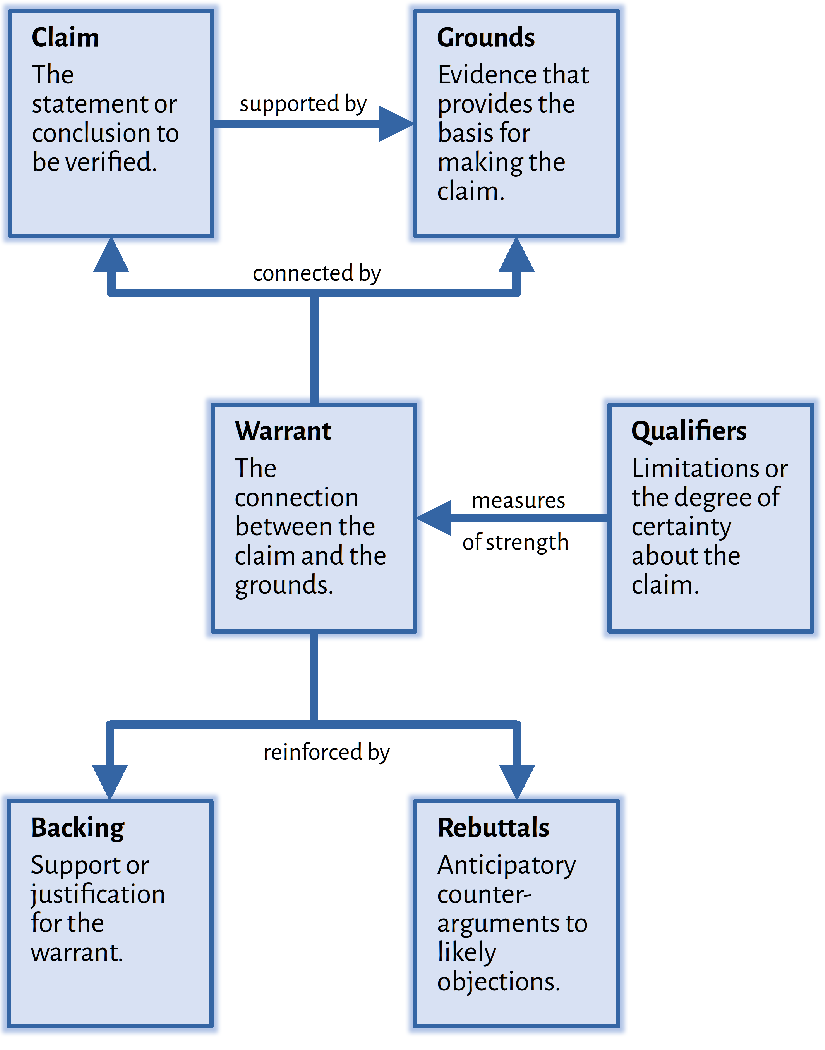
\includegraphics[width=0.75\textwidth] {Toulmin Argument Schema}}{Adapted from ``Toulmin Argument,'' Kalyca Schultz, Virginia Western Community College, CC-BY-SA in “Toulmin Argument Model” by Liza Long, Amy Minervini, and Joel Gladd is licensed under CC BY-NC-SA 4.0}
\end{figure}

\paragraph{Claim}
Rocketship is structured and operates to leverage various kinds of government funding (loans, grants, credit repair) to increase their real estate holdings which then allows it to open more charter schools.

\paragraph{Grounds}
Rocketship's main focus is not on academic success, but on acquiring real estate that is paid for by someone else. Several observations point in this direction.
\begin{itemize}
  \item How they have structured themselves, and  how they have funded themselves.
  \item What California law, their Articles of Incorporation, and IRS Code say about individual enrichment.
  \item How they spend their time and where they spend their money.
\end{itemize}

Right from the beginning, Rocketship separated the financing, acquisition, and operation of their facilities from the running of a school; they borrowed heavily and made extensive use of government programs to fund their real estate projects. Rocketship has not availed itself (except in one instance) of alternative ways of acquiring facilities. They have not used Proposition 39 to obtain classrooms and fields from a school's home district. They have not tried to convert commercial office space into classrooms. They have not modified existing buildings to serve as schools or classrooms. Instead they bought land and built a suitable school.

Since Rocketship and Launchpad, as nonprofit public benefit corporations, cannot distribute their income or assets according to law and to their Articles of Incorporation, they must have a different goal than enriching individuals. Rocketship Education's and Launchpad Development Company's Articles of Incorporation both contain language that is similar to, but more clearly expressed in ``Summit Public School's [Restated] Articles of Incorporation'':
\begin{quotation}\noindent%
Article III: The property of this Corporation is \textit{irrevocably} [emphasis added] dedicated to charitable purposes and no part of the \textit{net income or assets} [emphasis added] thereof or to the benefit of private persons except that the Corporation shall be authorized and empowered to pay reasonable compensation for services rendered and to make payments and distributions in furtherance of the purposes set forth in Article II of these Articles of Incorporation. \parencite[2]{SummitPublicSchools2017}
\end{quotation}
The Articles of Incorporation for both Rocketship and Launchpad are possibly equivalent to the first paragraph of Article III of Summit's quoted above, but they are not as explicit or definitive, and they are spread out over several articles and paragraphs.\footnote{Since both Rocketship and Summit make an exception to the prohibition of private gain for services rendered in their articles of incorporation, and entirely reasonable exception, and Launchpad's articles of incorporation do not, this raises the question of whether the \$300K salary of Launchpad's CFO \parencite[7]{zotero-16512} in 2019–2020, for example, violates Launchpad's Articles of Incorporation.} California and IRS code forbid distribution of income or assets to anything but another public benefit corporation (see \prettyref{sec:real-estate-conv} below), individual enrichment is illegal. 

Lastly, judging by the number of board committees devoted to non-academic topics, Rocketship leadership has spent most of their time on real estate issues.

\paragraph{Warrant}
The best indicator of a firm's real goals is not on what it says its goals are, but how it actually spends its time and on what it actually spends its money. 

\paragraph{Backing}
Time and money are both in limited supply, so firms must decide how to allocate their time and money, and this allocation reveals the firm's preferences and its goals.

\paragraph{Rebuttals}
A possible objection is that the three grounds given are neither necessary nor sufficient to prove the claim; there could be reasons other than the expansionary reasons given for Rocketship to have structured themselves they way they did. True, and also true, the way they spend their time and money could be not their choice, but instead due to outside constraints or being forced upon them. It is nonetheless hard to wish away governing law and the tax code. The first and third grounds are usually good indicators, but the second is unavoidable.

A second potential objection is that the warrant only addresses the third ground for making the claim, and doesn't support the first two grounds. True, but that objection overlooks the element of choice, one optional and one mandatory. Implied in the claim, the grounds and the warrant is that Rocketship had some level of choice in how they organized themselves. They could have chosen to make RSED (the parent organization) a 509(a)(3) supporting charity for individual 503(c)(3) nonprofit public benefit corporations that only provided requested services instead of forced management, or they could have even done away with RSED completely and just had a loose collection of independent charter schools. Instead they chose an organization that made RSED the decision maker and Launchpad the accumulator of value. As for the second ground for supporting the claim, Rocketship has no choice, unless their officers and members are willing to risk fines and potential jail time. Given the opposition and accompanying media exposure that some of their schools generated, that would be quite a bold risk to take.

\section{Answering the Research Question}%
\label{sec:answ-rese-quest}\indent%

As indicated above, this dissertation's research question is actually three sub-questions:
\begin{enumerate}
  \item Has Rocketship structured itself to make a profit?\footnote{Public benefit corporations (nonprofits) are allowed to make a profit, i.e. revenue exceeds expenses; they are, however, not allowed to \textit{distribute} that profit. Any profit must be use to further is public benefit purpose identified in their articles of incorporation.}
  \item If so, is real estate the vehicle that Rocketship uses to make money?
  \item Is this Rocketship's intent?
\end{enumerate}

The arguments given above indicate that the answers are: yes, yes, and yes.

Two questions remain: How and Why? It is not known how the owners and investors of Rocketship could convert the assets of Rocketship and Launchpad into transferable wealth. Perhaps they do not intend to. \prettyref{tab:type_conversion} below lists some of the forms and restrictions on converting real estate assets owned by a non-profit charter school.

\noindent%
\begin{table}[hbtp]
  \caption[Type of Conversion]{\textit{Type of Conversion}}%
  \label{tab:type_conversion}\OnehalfSpacing%
    \begin{tabulary}{\textwidth}{LLL}
    \toprule
    \textbf{Conversion Type} & \textbf{OK?} & \textbf{Notes} \\
    \midrule
    Excessive salaries & No & Listed in Form 990. Monitored by the IRS \vspace{6pt} \\
    Sale of assets to a private entity or for-profit corporation & No & Prohibited by CA Government Code, IRS Code, Articles of Incorporation. Requires AG notification \vspace{6pt} \\
    Arms-length transactions & Yes & Allowed by conflict of interest laws \vspace{6pt} \\
    Conversion of property to condos or apts. & No & Non-profits restricted to charitable purposes \\
    \bottomrule
  \end{tabulary}
\end{table}

That then begs the question of why Rocketship is accumulating assets. According to California law and to IRS Code, charter schools are not allowed to transfer money to a for profit entity or to private individuals. The option which makes the most sense in explaining Rocketship's structure and activities given the investments of Reed Hastings, Andre Agassi, the Walton Family Foundation, and others, all strong charter school supporters, is that Rocketship wants to become a self-sufficient pipeline of new charter schools for the entire United States. They have already expanded into Washington, D.C., Texas, Tennessee, and Wisconsin.

\section{Public Policy Issues}%
\label{sec:publ-policy-chang}\indent%

There are at least three major public policy issues that are raised by Rocketship's growth in assets and presumed expansion goals. First, are charter schools or charter school chains a net benefit to Californians? Secondly, is there too much opportunity for fraud, and lastly, should charter school chains in California use their assets (paid for by Californians) to create charter schools in other states? This last public policy issue could be more broadly construed to ask if any Californian tax dollars should leave the state with no benefit to Californians.

The first of these public policy issues, the net benefit of Californian charter schools to California, is beyond the scope of this dissertation because it would require a thorough analysis of not only the finances of charter schools, but also of the costs and benefits of the education they offer, their impact on public schools, and their impact on the communities they serve. The second and third issues—opportunities for fraud and creating charter schools in other states—are discussed in the sections below.

\subsection{Fraud}%
\label{sec:fraud}\indent%

The Association of Certified Fraud Examiners issues an annual \textit{A Report to the Nations} which is a global study on occupational fraud. Of interest is a diagram of the types of occupational fraud, reproduced below.
\begin{figure}[htbp]
  \caption{\textit{The Fraud Tree}}%
  \label{fig:fraud-tree}\centering%
  \copyrightbox[b] {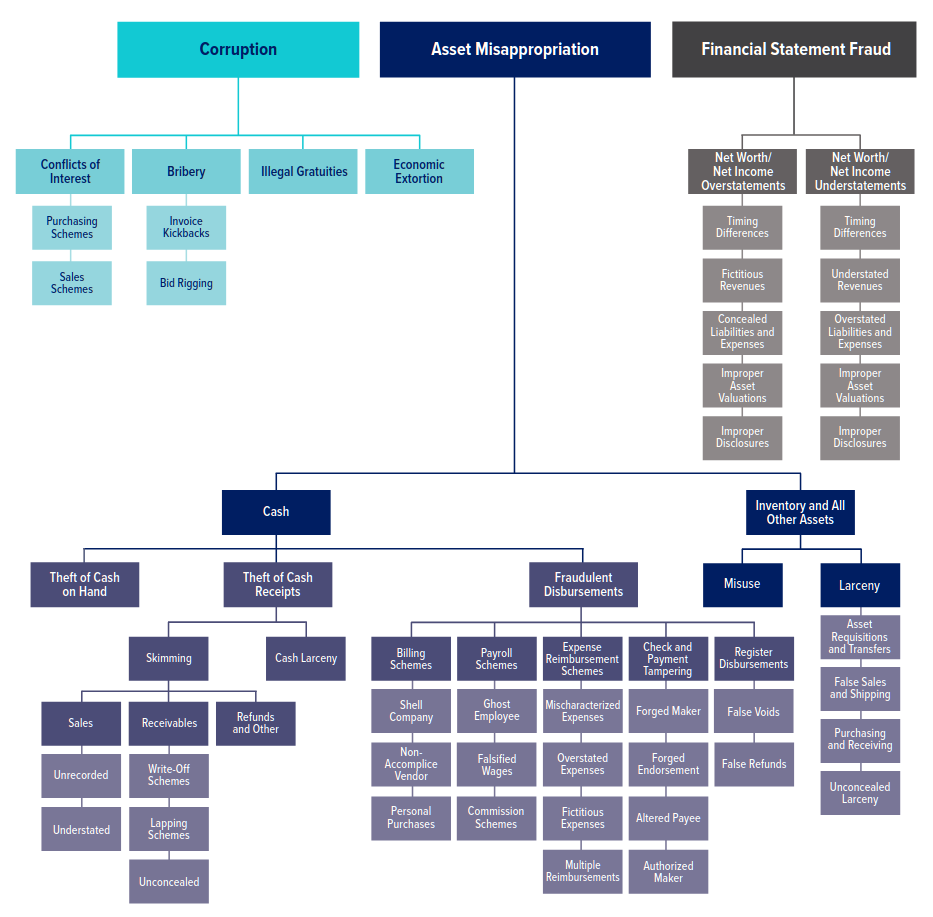
\includegraphics[width=0.85\textwidth]{2022 Report to the Nations-p.10}}
    {Reproduced by permission with attribution: \textit{Occupational Fraud 2022: A Report to the Nations.} Copyright 2022 by the Association of Certified Fraud Examiners, Inc.}
  \end{figure}
  The reason the Fraud Tree is interesting is because public policy should make sure that laws or regulations are in place to prevent all types of fraud from occurring. The diagram shows three major categories, eight immediate subcategories, and 47 specific types of occupational fraud, fraud that occurs in the context of employment. Note that much of this fraud can be eliminated by mandating robust internal controls and thorough, independent audits, neither of which are completely in place for charter schools. This should be an active area for new or modified legislation.

  Current California law and regulations are clearly insufficient to prevent massive fraud. The largest case so far involved the A3 Charter Schools in San Diego. The San Diego County District Attorney filed an 235 page indictment \parencite{SDDA2019} alleging a \$400M scheme to defraud the State of California. The two principle defendents pleaded guity \parencite{Taketa2021}.
  Seventeen years earlier, the California State Auditor found that not only did authorizers and the California Department of Education fail to meet the student outcomes their charter required, but fiscal oversight was insufficient \parencite{CAStateAuditor2002}. In 2021, the Network for Public Education issued a report on how charter schools across the United States profit from lax oversight and regulations \parencite{Burris.Cimarusti2021}. Essentially, CMOs ``sweep'' all of the revenues of a charter school chain in return for administration, management, and marketing services. These CMOs may be for-profit corporations in other states. In 2016, Kamala Harris, then the California Attorney General, announced a settlement with K12 of \$168.5M because misleading advertising and misreported attendance numbers \parencite{Agpressoffice2016}.

  Another area which is extremely difficult to monitor, as Justice Clarence Thomas has shown \parencite{Murphy.Mierjeski2023}, is gifts which do not involve the exchange of money, such as luxury vacations, private jet travel, and VIP passes to sporting events. These illegal gratuities leave no financial traces and it may be hard to establish that a \textit{quid pro quo} exists. 

  Some activities that are actually conflicts of interests can be masked so they appear as perfectly legal and normal. For example piloting EdTech software (Dreambox, Clever, Zeal Learning) is an activity that many public, private, and charter schools do, and this (in theory) improves the educational outcomes of students. But, if the founder of two EdTech companies (John Danner) was also the founder of Rocketship, there exists the possible of an appearance of a conflict of interest.
\footnote{ California conflict of interest law is complex \parencite{Chaney.etal2010a} and is beyond the scope of this dissertation.}

With billions of dollars in funding every year in California alone, with little accountability, it is not surprising that fraud occurs in California's charter schools. Despite this, there is no indication that Rocketship or its principals engaged in fraudulent activities. However, as noted below, unaccounted for expenditures leave open the possibility of private gain. 

\subsection{Real Estate Conversion}%
\label{sec:real-estate-conv}\indent%

In the Public Interest, a national research and public policy organization says in \textcite{ITPI2018}
\begin{quotation}
  Due to a loophole in [California] law, some private groups have used this public money to buy private property. While charter schools constructed with general obligation bonds cannot be sold or used for anything other than the authorized school, schools constructed with tax-exempt conduit bonds become the private property of the charter operator. Even if the charter is revoked, neither the state nor a local school district can take control of this property. Additionally, schools constructed with private funding subsidized by New Market Tax Credits or acquired with private funds but whose mortgage payments are reimbursed through the Charter Facilities Grant Program (known as “SB740”) are typically owned without restriction. In the event that such schools close down, their owners may be free to turn the buildings into condominiums or retail space, or sell them at a profit. In such cases, neither the school district nor any other public body is entitled to recoup the public dollars that have gone toward creating the facility. \parencite[6]{ITPI2018}
\end{quotation}

However, this is likely not correct because a plain reading of the law doesn't allow nonprofits to benefit private individuals.\footnote{Here are a few excerpts from IRS regulations and California law.
  
  \begin{itemize}[topsep=0.125\baselineskip,itemsep=0.25\baselineskip]
    \item The IRS says this about 501(c)(3) organizations under the heading "Exemption Requirements":
    \begin{quote}\noindent
      To be tax-exempt under section 501(c)(3) of the Internal Revenue Code, an organization must be organized and operated exclusively for exempt purposes set forth in section 501(c)(3), and none of its earnings may inure to any private shareholder or individual.
      \ldots\\
      The organization must not be organized or operated for the benefit of private interests, and no part of a section 501(c)(3) organization's net earnings may inure to the benefit of any private shareholder or individual.
    \end{quote}
    
    \item The California Attorney General says in \textit{Attorney General's Guide for Charities} (2021):
    \begin{quote}
      Under California law, a public benefit corporation must be formed for public or charitable purposes and may not be organized for the private gain of any person. A public benefit corporation cannot distribute profits, gains, or dividends to any person. (p.3)
    \end{quote}
    and
    \begin{quote}
      Although public benefit corporations may qualify for important benefits, including exemption from income tax, they are subject to important legal restrictions. One critical restriction is that the assets of a public benefit corporation are considered irrevocably dedicated to charitable purposes, and cannot be distributed for private gain. (p.7)
    \end{quote}
    Finally, the AG says on p.14, ```In addition, the founding document must require the organization to expressly dedicate its assets to exempt purposes in the event of dissolution.''
    \item California Code, §§ 5130, 5237, 5410. Section 5410 says "No corporation shall make any distribution."
  \end{itemize}}
Consequently, income and assets, during the lifetime of the nonprofit, or at dissolution, can only be transferred to other nonprofits, and at dissolution, a 20-day prior notice must be given to the California Attorney General. The prohibition of private gain and the requirement to notify the CA Attorney General rule out Rocketship converting its properties to condominiums or retail space. Lease payments under SB740 do continue even after any debt used to purchase real estate or to improve a property which has been paid off. This is an income stream that does not benefit Rocketship's children because it merely increases the value of Rocketship itself without funding any academic programs.

\newpage
\section{Areas for Future Research}%
\label{sec:areas-future-rese}\indent%

Rocketship records \$7.5M spent on travel in the four years of 2019–2022. Since this is a significant sum, a future investigation should ask for details to substantiate the propriety of those expenditures. Details like who traveled, what class did they travel in, where did the go and where did they come from. Since these travel expenditures appeared in an annual financial statement, the investigation might ask what object codes went into each of the categories listed in \prettyref{tab:consolidated_functional_expenses} on p.\pageref{tab:consolidated_functional_expenses}.

As far back as 2002, the California State Auditor said, 
  \begin{quote}
    Finding \#3: Chartering entities lacked policies and procedures for fiscal monitoring and have not adequately monitored their charter schools. \parencite{CAStateAuditor2002}
  \end{quote}
In other words, internal and external controls are lacking.

A study of what happened to a charter's assets when a charter dissolves is needed because, although the law says that nonprofits cannot benefit individuals, and nonprofits must notify the Attorney General at dissolution, there is no effective monitoring nor is any enforcement mechanism. The result is that we have no idea of what happened to the assets of the hundreds of charter schools which have closed since 1992.

Another area for future research is calculating the net benefit of charter schools. Many studies have been made that examine the academic performance of charter schools vs public schools, and some studies have been made which quantify some of the costs to public schools when a charter school opens, but I am not aware of any study that incorporates \textit{all} of the costs and benefits of charter schools, even for a single school district, much less for an entire state or for all of the United States.

One area that has not been adequately explored is the 26 sheet Excel spreadsheet that Rocketship used for forecasting and planning in 2009 (\url{https://docs.google.com/spreadsheets/d/1e5j8nn2Ofg6l5BlOaPi_qcByGH_OAt232RrvTkoJy2Q}). Some of its sheets forecast out to 2040, so it is clear that Rocketship is playing the long game. Understanding what Rocketship is thinking of doing would be revealed by a deep dive into this spreadsheet.

Finally, further research should examine in detail the \$2.6M spent on travel in 2022. 

\section{Conclusion}%
\label{sec:conclusion}\indent%

The conclusion this dissertation reaches is that Rocketship's finances do not and are not designed to benefit private individuals, but they are intended to benefit other nonprofit corporations, in particular, charter schools in states other than in California. If this is the case, then Californian taxpayers are effectively subsidizing charter schools in other states, a use of Californian tax dollars that I expect Californians would overwhelmingly reject.

Further, the differences in finances and especially accountability between public schools and charter schools admit the possibility for fraud in charter schools, a situation which is much less likely with the public school system because of their much greater transparency. It is difficult to prove that fraud has occurred, but it is even more difficult to prove that fraud has not occurred. Given the history of fraud in charter schools, and the amount of money which is sent to charter schools annually, and the lack of substantive financial controls and oversight, it would indeed be surprising if charter schools in California and Rocketship in particular were not engaged in some form or fraud.

%%% Local Variables:
%%% mode: latex
%%% TeX-master: "Rocketship_Education-An_Exploratory_Public_Policy_Case_Study"
%%% End: